
\documentclass[a4paper,11pt]{article}
\usepackage[a4paper, margin=8em]{geometry}

% usa i pacchetti per la scrittura in italiano
\usepackage[french,italian]{babel}
\usepackage[T1]{fontenc}
\usepackage[utf8]{inputenc}
\frenchspacing 

% usa i pacchetti per la formattazione matematica
\usepackage{amsmath, amssymb, amsthm, amsfonts}

% usa altri pacchetti
\usepackage{gensymb}
\usepackage{hyperref}
\usepackage{standalone}

% imposta il titolo
\title{Appunti Elettronica Digitale}
\author{Luca Seggiani}
\date{2026}

% imposta lo stile
% usa helvetica
\usepackage[scaled]{helvet}
% usa palatino
\usepackage{palatino}
% usa un font monospazio guardabile
\usepackage{lmodern}

\renewcommand{\rmdefault}{ppl}
\renewcommand{\sfdefault}{phv}
\renewcommand{\ttdefault}{lmtt}

% disponi il titolo
\makeatletter
\renewcommand{\maketitle} {
	\begin{center} 
		\begin{minipage}[t]{.8\textwidth}
			\textsf{\huge\bfseries \@title} 
		\end{minipage}%
		\begin{minipage}[t]{.2\textwidth}
			\raggedleft \vspace{-1.65em}
			\textsf{\small \@author} \vfill
			\textsf{\small \@date}
		\end{minipage}
		\par
	\end{center}

	\thispagestyle{empty}
	\pagestyle{fancy}
}
\makeatother

% disponi teoremi
\usepackage{tcolorbox}
\newtcolorbox[auto counter, number within=section]{theorem}[2][]{%
	colback=blue!10, 
	colframe=blue!40!black, 
	sharp corners=northwest,
	fonttitle=\sffamily\bfseries, 
	title=~\thetcbcounter: #2, 
	#1
}

% disponi definizioni
\newtcolorbox[auto counter, number within=section]{definition}[2][]{%
	colback=red!10,
	colframe=red!40!black,
	sharp corners=northwest,
	fonttitle=\sffamily\bfseries,
	title=~\thetcbcounter: #2,
	#1
}

% U.D.M
\newcommand{\amp}{\ensuremath{\mathrm{A}}}
\newcommand{\volt}{\ensuremath{\mathrm{V}}}
\newcommand{\meter}{\ensuremath{\mathrm{m}}}
\newcommand{\second}{\ensuremath{\mathrm{s}}}
\newcommand{\farad}{\ensuremath{\mathrm{F}}}
\newcommand{\henry}{\ensuremath{\mathrm{H}}}
\newcommand{\siemens}{\ensuremath{\mathrm{S}}}

% circuiti
\usepackage{circuitikz}
\usetikzlibrary{babel}

% disegni
\usepackage{pgfplots}
\pgfplotsset{width=10cm,compat=1.9}

% disponi codice
\usepackage{listings}
\usepackage[table]{xcolor}

\lstdefinestyle{codestyle}{
		backgroundcolor=\color{black!5}, 
		commentstyle=\color{codegreen},
		keywordstyle=\bfseries\color{magenta},
		numberstyle=\sffamily\tiny\color{black!60},
		stringstyle=\color{green!50!black},
		basicstyle=\ttfamily\footnotesize,
		breakatwhitespace=false,         
		breaklines=true,                 
		captionpos=b,                    
		keepspaces=true,                 
		numbers=left,                    
		numbersep=5pt,                  
		showspaces=false,                
		showstringspaces=false,
		showtabs=false,                  
		tabsize=2
}

\lstdefinestyle{shellstyle}{
		backgroundcolor=\color{black!5}, 
		basicstyle=\ttfamily\footnotesize\color{black}, 
		commentstyle=\color{black}, 
		keywordstyle=\color{black},
		numberstyle=\color{black!5},
		stringstyle=\color{black}, 
		showspaces=false,
		showstringspaces=false, 
		showtabs=false, 
		tabsize=2, 
		numbers=none, 
		breaklines=true
}

\lstdefinelanguage{javascript}{
	keywords={typeof, new, true, false, catch, function, return, null, catch, switch, var, if, in, while, do, else, case, break},
	keywordstyle=\color{blue}\bfseries,
	ndkeywords={class, export, boolean, throw, implements, import, this},
	ndkeywordstyle=\color{darkgray}\bfseries,
	identifierstyle=\color{black},
	sensitive=false,
	comment=[l]{//},
	morecomment=[s]{/*}{*/},
	commentstyle=\color{purple}\ttfamily,
	stringstyle=\color{red}\ttfamily,
	morestring=[b]',
	morestring=[b]"
}

% disponi sezioni
\usepackage{titlesec}

\titleformat{\section}
	{\sffamily\Large\bfseries} 
	{\thesection}{1em}{} 
\titleformat{\subsection}
	{\sffamily\large\bfseries}   
	{\thesubsection}{1em}{} 
\titleformat{\subsubsection}
	{\sffamily\normalsize\bfseries} 
	{\thesubsubsection}{1em}{}

% disponi alberi
\usepackage{forest}

\forestset{
	rectstyle/.style={
		for tree={rectangle,draw,font=\large\sffamily}
	},
	roundstyle/.style={
		for tree={circle,draw,font=\large}
	}
}

% disponi algoritmi
\usepackage{algorithm}
\usepackage{algorithmic}
\makeatletter
\renewcommand{\ALG@name}{Algoritmo}
\makeatother

% disponi numeri di pagina
\usepackage{fancyhdr}
\fancyhf{} 
\fancyfoot[L]{\sffamily{\thepage}}

\makeatletter
\fancyhead[L]{\raisebox{1ex}[0pt][0pt]{\sffamily{\@title \ \@date}}} 
\fancyhead[R]{\raisebox{1ex}[0pt][0pt]{\sffamily{\@author}}}
\makeatother

\begin{document}
% sezione (data)
\section{Lezione del 03-03-26}

% stili pagina
\thispagestyle{empty}
\pagestyle{fancy}

% testo
\subsection{Conduzione}
Iniziamo a dettagliare il fenomeno della conduzione attraverso un materiale.
Supponiamo di avere un parallelepipedo di sezione $S$ e lunghezza $L$.

\begin{theorem}{Seconda legge di Ohm}
Dalla seconda legge di \textit{Ohm}, la sua abilità di condurre cariche di un corpo è inversamente proporzionale alla \textbf{resistenza}:
$$
R = \rho \frac{L}{S}
$$
\end{theorem}
dove $\rho$ è una costante specifica al materiale detta \textit{resistività}.
Ricordiamo che questo deriva dalla formulazione propria di quella che chiameremo legge di \textit{Ohm microscopica}:
$$
J = \sigma E
$$
dove $J$ è la \textit{densità di corrente} e $\sigma$ è la \textit{conducibilità} di un materiale, per cui:
$$
I = JS = \sigma E S = \frac{1}{\rho} \frac{V}{L} S = \frac{V}{R}
$$
dove si è usato la definizione di \textit{potenziale elettrico} $V = EL$ sulla distanza $L$.

Abbbiamo quindi ricavato la legge:
\begin{theorem}{Prima legge di Ohm}
Differenza di potenziale, corrente e resistenza sono legate dalla relazione:
$$
V = IR
$$
\end{theorem}

Riguardo a resistività e conducibilità, le cui unità di misura sono rispettivamente $\Omega \cdot \mathrm{cm}$ e $\Omega \cdot \mathrm{cm}^-1$, vale la relazione:
$$
\rho = \frac{1}{\sigma}
$$
immediata dalla definizione a partire dalla legge di Ohm.

\subsubsection{Conduttori, semiconduttori e isolanti con Ohm}
Sulla base della resistività si possono classificare i materiali in \textit{conduttori}, \textit{semiconduttori} e \textit{isolanti} come accennato in 1.2.2.

In particolare, si riporta la tabella che individua i valori di resistività per diversi tipi di materiale:
\begin{table}[h!]
	\center \rowcolors{2}{white}{black!10}
	\begin{tabular} { c | c }
		\bfseries Tipo & \bfseries Resistività \\
		\hline
		Conduttore & $\rho < 10^{-2} \, \Omega \cdot \mathrm{cm}$ \\
		Isolante & $\rho > 10^5 \, \Omega \cdot \mathrm{cm}$ \\
		Semiconduttore & $10^{-2} \, \Omega \cdot \mathrm{cm}< \rho < 10^5 \, \Omega \cdot \mathrm{cm}$ \\
	\end{tabular}
\end{table}

Il vantaggio dei materiali semiconduttori, su cui noi ci concentriamo (in particolare noi assumiamo di usare il \textit{silicio}, simbolo atomico \textit{Si} e numero atomico 14) è che la loro resistività può essere controllata in maniera tale da decidere se in una data occasione un semiconduttore deve comportarsi come un isolante o come un conduttore (come abbiamo accennato, il processo di \textit{drogaggio} di 1.2.2).

\subsubsection{Corrente di deriva in un conduttore}
La \textbf{corrente di deriva} è quella che otteniamo applicando un campo elettrico $\vec{E}$ ad un materiale.

Riprendiamo il parallelepipedo di 2.1, e assumiamo che sia composto da un materiale conduttore ($\rho < 10^{-2} \, \Omega \cdot \mathrm{cm}$).

Prendiamo la definizione di corrente come quantità di carica che si sposta in una superficie nell'istante di tempo, cioè:
$$
I = \frac{\Delta Q}{\Delta T}
$$
Questo per noi significherà prendere una sezione del parallelepipedo e "contare" il numero di cariche che vi passano attraverso.

\par\smallskip

\noindent
\textbf{\textsf{Modello di Drude-Lorentz}}

\noindent
Il modello di \textit{Drude-Lorentz} si pone di studiare il fenomeno della conduzione considerando quindi queste cariche libere all'interno di un metallo (prendiamo ad esempio il rame, che con configurazione elettronica $[\mathrm{Ar}]3d^{10}4s^1$ offre un elettrone libero per atomo) come particelle di un gas perfetto.

\begin{itemize}
	\item 
Se non si applica nessun campo $\vec{E}$, la corrente di deriva che passa attraverso il parallelepipedo sarà chiaramente 0. Notiamo che questo non deriva dal fatto che le cariche sono ferme, ma che si stanno muovendo in direzione casuale (e quindi statisticamente attraverso la nostra superficie entrano tante cariche quante ne escono).
	\item
Procediamo quindi ad applicare un certo campo $\vec{E}$.
Dalla definizione di campo elettrico, si ha che le cariche vengono sottoposte ad una forza (e rispettiva accelerazione) data da:
$$
\vec{F} = - e \vec{E}, \quad \vec{a} = - \frac{e \vec{E}}{m}
$$

Le traiettorie descritte dagli elettroni sono casuali, localmente in moto rettilineo uniforme finché questi non urtano altri elettroni. All'istante dell'urto modellizziamo la variazione di velocità (trascurando la forza relativa all'urto stesso) come:
$$
\vec{v}_{i + 1} = \vec{v}_i - \frac{e \vec{E}}{m} \tau
$$
dove $\tau$ è il tempo necessario ad effettuare un \textit{cammino libero medio} all'interno del conduttore.

Si ha quindi che la \textbf{velocità di deriva} media sarà data da:
$$
\vec{v}_d = < \vec{v}_{i + 1} > = - \frac{e \vec{E}}{m} \tau
$$
\end{itemize}

Dal punto di vista macroscopico, quello che avremo è che la velocità media è legata ad un parametro $\mu_m$ detto \textit{mobilità}, e direttamente proporzionale al campo:
$$
\vec{v}_d = -\mu_m \vec{E}
$$
dove ricordiamo il segno negativo, in quanto gli elettroni si muovono nella direzione opposta al campo (sono cariche negative $-1 \, e$).

\par\smallskip

\noindent
\textbf{\textsf{Da Drude-Lorentz a Ohm}}

\noindent
Vediamo come riagganciarci alle leggi di Ohm a partire dal modello di Drude-Lorentz appena visto.

Osserviamo il percorso di una singola carica nel nostro materiale conduttivo, e prendiamo il tempo che impiega a passare da un capo all'altro del materiale come:
$$
\Delta T = \frac{L}{\vec{v}_d}
$$
detto \textit{tempo di osservazione}. Riprendendo la definizione di corrente, e supponendo che nel materiale siano presenti $N$ cariche elettroniche, potremo quindi dire:
$$
I = \frac{\Delta Q}{\Delta T} = \frac{e N}{\Delta T} = \frac{e N}{L} v_d
$$

Ci possiamo riportare anche alla densità di corrente $J$ ponendo:
$$
J = \frac{I}{S} = \frac{e N v_d}{LS} = \frac{e N v_d}{V_{ol}} 
$$
dove $V_{ol} = LS$ è il \textit{volume} del parallelepipedo.
Chiamiamo quindi $n$ la \textit{concentrazione} di carica all'interno del volume:
$$
n = \frac{N}{V_{ol}}
$$
in modo da poter dare quello che sarà il nostro nodo chiave tra il modello di Ohm e quello di Drude-Lorentz:
\begin{definition}{Legge microscopica di Ohm}
La densità di carica in un materiale sottoposto ad un campo elettrico di modulo $E$ è:	
$$
J = \frac{N}{V_{ol}} e v_d = n e v_d = n e \mu_n E
$$
\end{definition}
\noindent
trascurando i segni (cioè assumendo che il campo sia perpendicolare al parallelepiedo conduttore considerato da principio).

Dal punto di vista vettoriale, riprendiamo la definizione della legge di Ohm, stavolta contando i segni:
$$
\vec{J} = \sigma \vec{E}, \quad \sigma = n (- e) \cdot (- \mu_n) = n e \mu_n 
$$
dove si applica sempre la relazione con la resistività:
$$
\rho = \frac{1}{\sigma} = \frac{1}{n e \mu_n}
$$

\newpage

Notiamo che appunti più accurati e tratti da un corso di fisica su questo argomento si possono trovare a \url{https://raw.githubusercontent.com/seggiani-luca/appunti-fis/68a83a26dacd1f545dcf697da0daabf257413325/master/master.pdf}. In particolare, negli appunti riportati si derivano completamente resistività e conduttività nel contesto del modello di Drude-Lorentz, oltre alla legge microscopica di Ohm (pagina 149).

In particolare, si mantiene la mobilità degli elettroni $\mu_e$ in funzione delle caratteristiche del materiale e del tempo di cammino libero medio $\tau$:
$$
\vec{v}_d = -\frac{e \vec{E}}{m} \tau = - \mu_m \vec{E} \implies \mu_m = \frac{e \tau}{m}
$$
che sostituito nei nostri risultati dà la stessa cosa:
$$
\rho = \frac{m}{n e^2 \tau}, \quad \sigma = \frac{1}{\rho} = \frac{n e^2 \tau}{m}
$$

\par\smallskip

Abbiamo quindi derivato le leggi di Ohm a partire dalla densità di carica, e abbiamo visto come questa necessita solamente della conoscenza delle cariche libere in un materiale e la loro velocità di deriva. 

Il modello di Drude-Lorentz ci permette quindi di stimare tale velocità di deriva, a partire da una visione delle particelle basata sulla meccanica classica e sulla forza di Lorentz applicata alle cariche. 

\par\smallskip

\noindent
\textbf{\textsf{Esempio numerico col rame}}

\noindent
Fissiamo i concetti visti nell'ultima sezione con un esempio numerico. Poniamo di voler calcolare, a partire dal modello di Drude-Lorentz, la resistività del rame.
Avevamo la formula:
$$
\rho = \frac{m}{n e^2 \tau}
$$
e del rame conosciamo i valori:
\begin{table}[H]
	\center \rowcolors{2}{white}{black!10}
	\begin{tabular} { c | c | c  }
		\bfseries Quantità & \bfseries Simbolo & \bfseries Valore \\
		\hline 
		Massa dell'elettrone & $m$ & $9.11 \times 10^{-31} \, \mathrm{kg}$ \\
		Densità atomica del rame & $n$ & $8.47 \times 10^{28} \, \frac{\text{atomi}}{\mathrm{m}^3}$ \\
		Carica dell'elettrone & $e$ & $1.6 \times 10^{-19} \, \mathrm{C}$ \\ 
		Tempo di cammino libero medio & $\tau$ & $2.5 \times 10^{-14} \, \mathrm{s}$ 
	\end{tabular}
\end{table}
per cui:
$$
\rho = \frac{9.11 \times 10^{-31}}{8.47 \times 10^{28} \cdot \left( 1.6 \times 10^{-19} \right)^2 \cdot 2.5 \times 10^{-14}} = 1.68 \times 10^{-8} \, \Omega \cdot \mathrm{m}
$$
che si allinea coi risultati sperimentali e classifica il rame come un ottimo conduttore, secondo quanto detto in 2.1.1.

\subsubsection{Corrente di deriva in un semiconduttore}
Negli scorsi esempi riguardo alla corrente di deriva abbiamo fatto uso di un materiale conduttore (in particolare del rame). In un semiconduttore, la situazione cambia in quanto i legami che si formano fra gli atomi non sono più metallici.

\begin{center}
	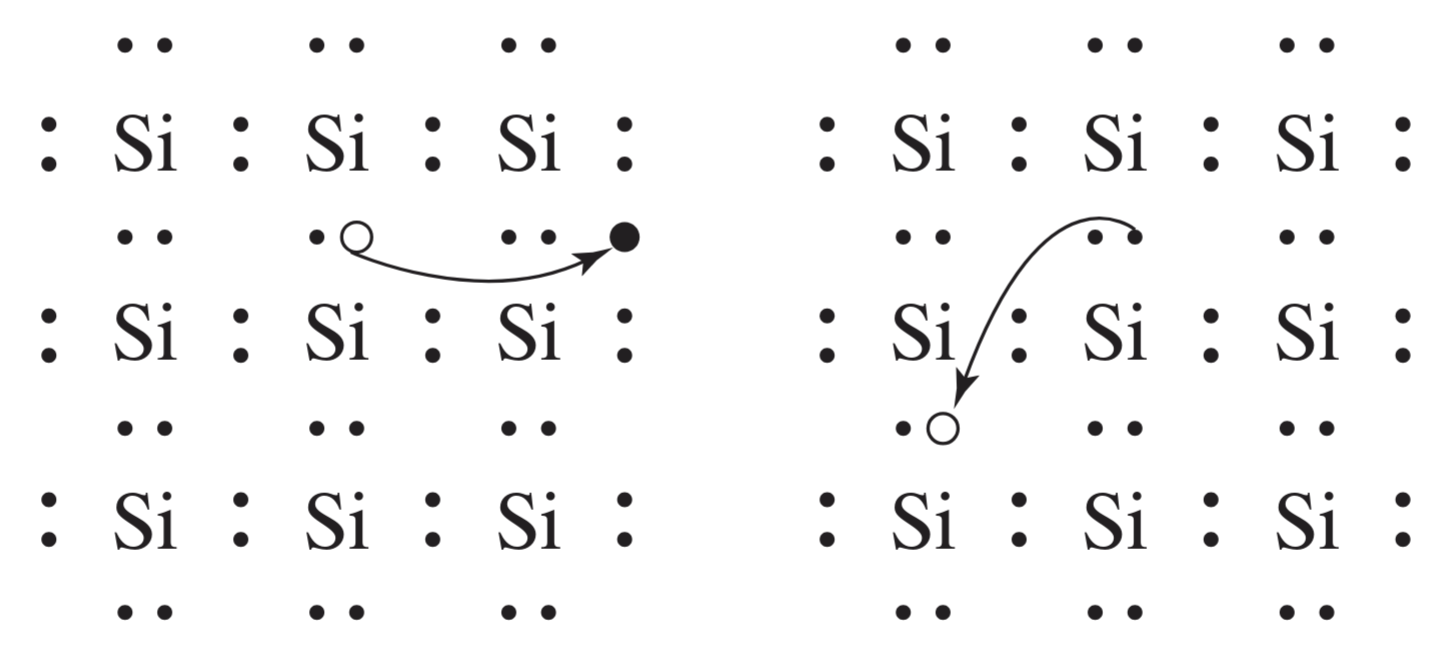
\includegraphics[scale=0.15]{../figures/silicon_2d.png}
\end{center}

Prendiamo ad esempio il silicio, che forma legami di tipo covalente. Abbiamo detto in 1.2.3 che il silicio presenta 4 elettroni nello strato di valenza, per cui è capace di formare legami covalenti con altri 4 atomi di silicio in una struttura cristallina tidimensionale.
Gli elettroni nel reticolo cristallino del silicio saranno quindi costretti a trovarsi nella zona del legame fra gli atomi, e non potremo usare l'approssimazione a gas perfetto valida per i metalli. La chiave sarà quindi data dalla \textbf{temperatura}.

\begin{itemize}
	\item 
Di base, in una situazione dove la temperatura è $T = 0 \, \mathrm{K}$ gradi Kelvin, gli elettroni non sono liberi di muoversi nel reticolo e non si ha conduzione;
	\item 
Se invece si pone $T \neq 0 \, \mathrm{K}$, si può avere conduzione attraverso gli elettroni liberi che vengono "portati" via dal legame. Questo è reso possibile dal fatto che l'energia fornita come aumento di temperatura all'atomo è tale da superare l'energia di legame, e quindi liberare un elettrone coinvolto nel legame.
\end{itemize}

\par\smallskip

\noindent
\textbf{\textsf{Elettroni liberi in un semiconduttore}}

\noindent
Avremo quindi bisogno di un modello per il numero di elettroni liberi in funzione della temperatura.

\begin{theorem}{Statistica degli elettroni liberi in un semiconduttore intrinseco}
La densità di elettroni liberi in un semiconduttore intrinseco in funzione della temperatura $T$ è data da:
$$
n_i = B T^\frac{3}{2} e^{-\frac{E_G}{2 k_B T}}
$$
\end{theorem}
Ad esempio, abbiamo che a $300 \, \mathrm{K}$ gradi Kelvin, il numero di elettroni liberi nel silicio è circa $10^{10} \, \mathrm{cm}^{-3}$.

Nella legge riportata $n_i$ è la densità di elettroni liberi (analoga alla $n$ dei conduttori), $B$ è una costante dipendente dai materiali, $E_G$ è l'\textit{intervallo di banda} fra le cosiddette bande di \textit{valenza} e \textit{conduzione}, e $k_B$ è una costante detta costante di \textit{Boltzmann}.

Il modello che adottiamo per la statistica deriva dalla \textit{teoria delle bande}, dove si ipotizza che in un sistema di particelle come quello del silicio intrinseco ad ognuna può essere associato un livello energetico (non necessariamente corrispondente ai livelli energetici degli elettroni negli orbitali). Questo livello energetico non può essere conosciuto per ogni particella, ma si possono fare delle \textit{statisitche}. Riguardo all'intervallo di banda, abbiamo che tutti gli elementi presentano un livello energetico detto \textit{livello di Fermi} necessario a fornire o sottrarre elettroni. Due bande, dette appunto banda di valenza e banda di conduzione, si trovano rispettivamente sotto e sopra tale livello.

\begin{center}
	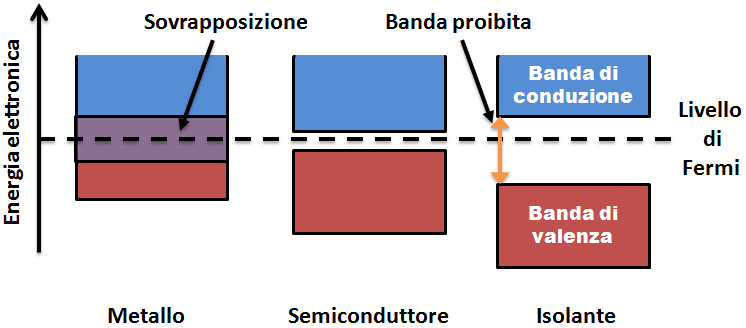
\includegraphics[scale=0.575]{../figures/proib.png}
\end{center}

\begin{itemize}
	\item Nei \textbf{conduttori}, la banda di valenza e la banda di conduzione si sovrappongono, o comunque è presente un \textit{intervallo di banda} $E_G$ (cioè la distanza fra le due bande) molto piccolo;
	\item Negli \textbf{isolanti}, le bande di valenze e la banda di conduzione sono molto distanti (l'intervallo di banda $E_G$ è consistente);
	\item Nei \textbf{semiconduttori} l'intervallo di anda $E_G$ è intermedio fra conduttore e isolante: come abbiamo visto, compare nella formula per la densità di elettroni liberi $n_i$, dove crescendo diminuisce $n_i$ in maniera esponenziale.
\end{itemize}

Capire il numero di portatori liberi equivale quindi a determinare una statistica per i livelli energetici e capire la probabilità che questi vadano a trovarsi nella zona di conduzione.
\begin{itemize}
	\item La statistica applicabile in questo caso sarebbe quella di \textit{Fermi-Dirac}, che in breve è:
$$
f_\text{Fermi-Dirac} \left(E\right)=\frac{1}{e^{\frac{\left(E-E_{F}\right)}{k_BT}}+1}
$$
	Questa restituisce la probabilità che una particella si trovi allo stato energetico $E$ (abbia energia $E$) rispetto al livello di Fermi $E_F$;
\item Nel caso $E - E_F >> k_B T$ si può semplificare adottando la statistica di \textit{Maxwell-Boltzmann}. Questa è una statistica adatta a particelle a temperatura più alta, basata sulla meccanica classica:
$$
f_\text{Maxwell-Boltzmann} \left(E\right)=e^{-\frac{\left(E-E_{F}\right)}{k_BT}}
$$
\end{itemize}

Vediamo su un grafico la differenza fra le statistiche $f_\text{Fermi-Dirac} \left(E\right)$ e $f_\text{Fermi-Dirac} \left(E\right)$, mettendo in evidenza la similarità per grandi valori di $E$:
\begin{center}
	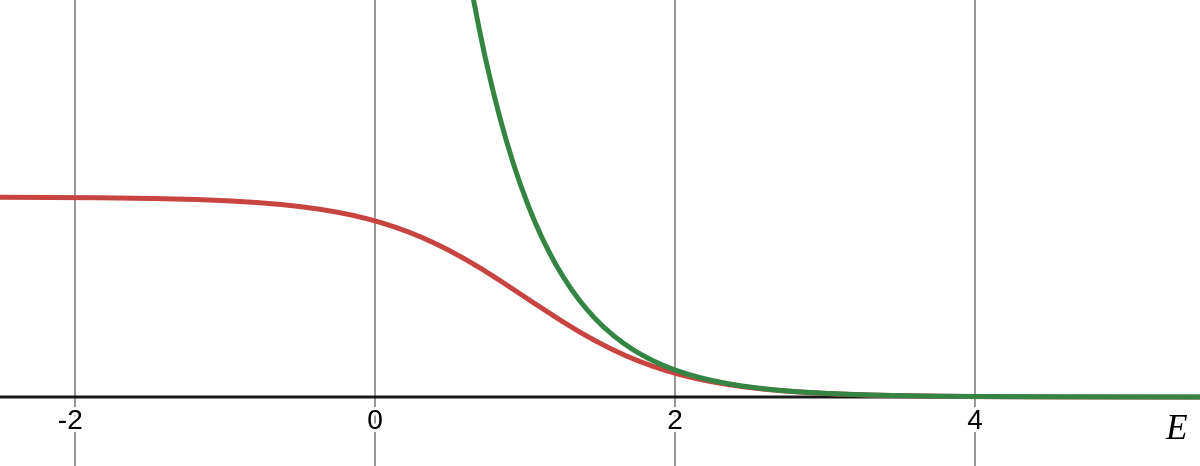
\includegraphics[scale=0.25]{../figures/statistics.png}
\end{center}

Per ricavare la formula in 2.2, quindi, prendiamo come livello $E = E_C$ alla base della banda di conduttività (questo è valido in quanto la maggior parte dei conduttori si concentra a tale livello). Se si ha che l'intervallo $E_G$ è più o meno centrato sul livello di Fermi, seguirà che:
$$
E_C - E_F = \frac{E_G}{2}
$$
che è ciò che troviamo nella formula. 
Infine, per il termine $B T^\frac{3}{2}$, abbiamo che questo deriva sempre dalla statistica di Maxwell-Boltzmann. In particolare, abbiamo che il termine $f_\text{Maxwell-Boltzmann} \left(E\right)$ indica la \textit{probabilità} di stati, mentre si dimostra che la \textit{densità} effettiva di stati va esponenzialmente (di fattore $\frac{3}{2}$) con la temperatura. Il prodotto fra questi darà la densità di particelle nel livello energetico di conduzione. 

\par\smallskip

Diciamo quindi che il silicio è un semiconduttore \textbf{intrinseco} in quanto ha naturalmente bassa conduttività. Di un semiconduttore drogato per ottenere maggiore conduttività si dice che è invece \textbf{estrinseco}. 

Vedremo che in diversi casi, trattando di conduttori estrinseci (per noi principalmente il silicio drogato) stabiliremo relazioni matematiche che faranno riferimento al comporamento di tali semiconduttori in condizioni intrinseche. In questo, $n_i$ si riferisce alla densità di elettroni liberi (come vedremo fra poco, di \textit{coppie lacuna-elettrone}) nel silicio intrinseco (che obbedisce a $n = p = n_i$ e vale circa $10^{10} \, \mathrm{cm}^{-3}$ a 300 Kelvin). 

\par\smallskip

\noindent
\textbf{\textsf{Generazione e ricombinazione termica}}

\noindent
Vediamo le condizioni di equilibrio del numero di elettroni liberi in un semiconduttore.

\begin{itemize}
	\item 
Il fenomeno visto finora prende il nome di \textbf{generazione termica} di elettroni liberi, in quanto chiaramente richiede di fornire calore al materiale semiconduttore le cui proprietà di conduzione vogliamo variare, in modo che questi si spostino nella fascia di conduzione;
	\item
Si può osservare anche il fenomeno opposto, detto di \textbf{ricombinazione termica}, quando un elettrone perde energia e decade nuovamente, dalla fascia di conduzione, in un legame covalente.
\end{itemize}

Si ha che la quantità effettiva di elettroni liberi deriva da entrambi i fenomeni (che ricordiamo essere entrambi dipendenti esclusivamente dalla temperatura), per cui a grandi linee:
$$
n_i = \text{generazione termica} + \text{ricombinazione termica}
$$
cioè due processi attivi, uno di generazione, e uno di ricombinazione, sono in corso in un semiconduttore. Chiaramente, il primo porta alla formazione di più elettroni liberi, mentre il secondo annichilisce quelli già formati. Se il nostro obiettivo è quello di migliorare le proprietà di conduzione di un semiconduttore, preferiremo il primo. 

Quanto abbiamo detto prima riguardo alle statistiche sui livelli energetiche vale quando ci si trova in condizioni di equilibrio dei processi di generazione e ricombinazione termiche. Questi sono infatti sempre in corso, e quando si stabilizzano le statistiche (e il numero di portatori liberi) diventa costante.
In particolare, se chiamiamo $G$ la frequenza di generazione termica, e $R$ la frequenza di ricombinazione termica, si trova una condizione di equilibrio a:
$$
G = R
$$
che per il silicio ci dà il valore di $10^{10} \, \mathrm{cm}^{-3}$ a 300 Kelvin.

\newpage

\noindent
\textbf{\textsf{Lacune elettroniche}}

\noindent
Un fenomeno che non abbiamo visto è quello comportato dal fatto che un elettrone che viene liberato da un legame forma una \textbf{lacuna} o \textit{vacuità} nel reticolo cristallino, cioè una regione di "vuoto" della carica.
Le lacune possono spostarsi come gli elettroni, in quanto semplicemente può cambiare il legame su cui la lacuna si trova. 
In questo modo può essere più semplice considerare le lacune come cariche positive ($+1 \, e$) che si spostano all'interno del reticolo cristallino al pari degli elettroni.

In verità, le lacune elettroniche nei semiconduttori sono importanti quanto gli elettroni, e abbiamo quindi 2 possibili trasportatori di carica:
\begin{itemize}
	\item Gli \textbf{elettroni}, che hanno carica $-1 \, e$. Ne indichiamo la densità con $n$;
	\item Le \textbf{lacune}, che hanno carica $+1 \, e$. Ne indichiamo la densità con $p$.
\end{itemize}

Abbiamo quindi l'immagine completa del fenomeno:
\begin{itemize}
	\item 
La \textit{generazione termica} dirà che, fornito calore ad un atomo di silicio, elettroni possono liberarsi dai loro legami covalenti spostandosi nella fascia di conduzione, e formando allo stesso tempo una lacuna elettronica. In un conduttore intrinseco, quindi, le coppie $(-1 e, +1 e)$ di elettroni e lacune vanno di paripasso;
	\item 
Allo stesso modo, la \textit{ricombinazione termica} sarà il fenomeno di ricadimento degli elettroni dalla fascia di conduzione ad uno dei legami covalenti della struttura cristallina del silicio. Si ha quindi che la coppia $(-1 e, +1 e)$ di elettrone e lacuna viene annichilita.
\end{itemize}

Notiamo quindi che, secondo quanto detto sull'equilibrio di formazione di coppie elettrone/lacuna, e il fatto che queste in tale equlibrio sono sempre in coppia, riguardo alle densità di elettroni liberi e lacune elettroniche in un semiconduttore intrinseco vale:
$$
n = p = n_i
$$

Possiamo quindi riportarci alla legge di Ohm, dando una definizione della conduttività di un elemento semiconduttore basata su elettroni e lacune:
$$
\sigma = n \mu_n e + p \mu_p e
$$
dove $\mu_p$ è la \textit{mobilità delle lacune}, che notiamo differisce da quella degli elettroni (già introdotta come $\mu_n$). In generale, la differenza fra la mobilità dell'elettrone e quella delle lacune sarà quella che ci permettera di variare la conduttività agendo sull'equilibrio stesso di elettroni e lacune, secondo il processo già accennato di cosiddetto \textit{drogaggio}.

\end{document}
